\chapter{Asking Wealthy Americans How They Got Rich (Palm Beach)}

This chapter follows a School of Hard Knocks field interview, curated by LazyingArt LLC, in which Palm Beach is treated not as scenery but as an instrument. We are given no blackboard, no settled classroom sequence, and no durable mathematical screenshots. Instead we are given refusals, sudden openings, a few hard numbers, and then a set of compact commercial laws: capital must move, spending has a replacement cost, value in the marketplace is distributed unequally because value delivered is distributed unequally, fear is not removed but acted through, and scale appears only when the entrepreneur ceases to be merely an operator.

\begin{remark}
No validated mathematical screenshots survive for this lecture. Every equation and diagram below is therefore transcript-backed, and where the transcript is unstable we keep the formalism schematic rather than pretending to recover more than is there.
\end{remark}

\section{Palm Beach as a billionaire field}

The lecture begins with a teaser montage whose function is scale, not argument. A yacht appears before the business behind it. Tony Robbins appears before the story that formed him. A celebrity-access beat appears before the interview itself. Even one quantitative marker arrives in teaser form: Tony Robbins says the first million came at age twenty-four, while the billionaire threshold came only recently. The viewer is meant to feel magnitude before being told what question will govern the day.

Then the first real event is a failure. A promised Jake Paul access point turns into a credentials problem, security steps in, and the host is forced back into the street. That failure is not ornamental. It tells us how the whole inquiry will proceed. Access is itself the first technical obstacle.

Only after this do we receive the formal field-setting. Palm Beach is announced as a billionaire playground, and the method is stated plainly: cold-approach wealthy people in public and ask how they got rich. A run of brief encounters follows. Some people walk on. Some refuse the camera. One retired racing driver offers only a compressed maxim: persistence. The content is still thin, but the rhythm is now established. Knowledge in this lecture will be extracted by approach, refusal, reset, and renewed approach.

\section{The yacht owner and capital in motion}

The first real opening comes at the waterfront, after the host hears of a yacht gathering and resolves not to leave without an answer. The owner of a large yacht says only that he is in the car business and has been there a long time. Then the scale of the object is fixed numerically:
\begin{equation}
P_{\text{yacht}} = 120\times 10^{6}\ \text{euros}.
\end{equation}
The host misreads the number in the moment, and a later line about single-year earnings is too unstable to formalize. We therefore keep the yacht price and discard the noisier claim.

What matters is not merely that the yacht is expensive. The lecture uses the object to force a practical question: what sort of capital process sustains possessions of this magnitude? The owner's answer is direct. At age seventy-eight he still works every day, still buys companies, and still thinks of retirement as premature. The crucial doctrine comes when he turns to money itself: many people hoard it, like looking at a bank balance for reassurance, but money sitting in the bank does not make money. It must be put to use.

A cautious reconstruction of the mechanism is
\begin{equation}
r_{\text{deploy}} > r_{\text{idle}},
\end{equation}
where \(r_{\text{idle}}\) is not a measured rate from the lecture but a name for parked capital, and \(r_{\text{deploy}}\) names the state in which cash has been attached to businesses, assets, and operating decisions. The examples he gives are concrete rather than textbook-like: buying businesses, buying boats, keeping money moving.

The same interview also contains a rough warning about scale. The opening of the sentence is garbled in the transcript, but the stable image is clear enough: one can put only so much food in the mouth before choking. The commercial analogue is that people often try to take on more than their present structure can carry.

\subsection{Question \& Answer}

\paragraph{Question.} Why does parked cash fail to build more wealth?

\paragraph{Answer.} Because in the lecture's logic cash is not wealth by mere visibility. It becomes productive only when it is attached to a process that can return more than it consumes. The difference is not decorative. It is structural: an admired balance is inert, but deployed capital enters circulation and can generate a new balance.

The owner's later anecdote about old loan books is compressed and unstable in wording, but its direction is still clear. Debt was once part of the path; repayment mattered; then the preference shifted toward using his own money rather than living indefinitely off borrowed structure. The stable lesson is therefore not a formula about leverage. It is the insistence that capital be disciplined and active rather than ornamental.

\section{Private equity, replacement cost, compounding, and follow-up}

Back on the street the lecture reaches its first long operational interview. A G-Wagon owner says he is in ``the money business,'' by which he means private equity. The exact company count is unstable, so we retain only the safe lower bound and the large personal-business figure:
\begin{align}
N_{\text{PE}} &> 80,\\
G_{\text{PE,personal}} &> \$3\times 10^{9}.
\end{align}
Here \(G_{\text{PE,personal}}\) is written as a generated amount rather than a valuation, because the transcript gives generation language but not a clean accounting category.

The interview becomes technical almost immediately. Asked what one financial principle he would leave to his children, the speaker gives the most compact arithmetic rule in the lecture: if you spend one dollar, you have to go make two. We may encode the rule as
\begin{equation}
E_{\text{replace}}(S)=2S.
\end{equation}
This is not meant as literal bookkeeping. It is a severity rule. Spending destroys more than a visible unit of cash; it destroys a growth position and therefore must be respected more heavily than its face value suggests.

\paragraph{Worked example.} If
\[
S=\$1{,}000,
\]
then the lecture's rule becomes
\[
E_{\text{replace}}(S)=2S=\$2{,}000.
\]
We should not read this as a theorem of accounting. We should read it as a discipline device: the spender must recover the outflow and rebuild the position from which further accumulation could begin.

The speaker then moves, in the transcript's own order, from spending to saving and from saving to compounding. He does not write a standard compound-interest formula, and we should not insert one. His point is narrower and more practical. Private equity is attractive because capital can compound inside businesses, but one must first save enough to enter the game. Capital is required before compounding becomes available.

Then comes a second pivot. Why keep building businesses once the numbers are already enormous? His answer is not mathematical at first. Business is fun. People are fun. Fulfillment is the number one deal. One must love what one does. The lecture keeps this motivational beat because it prepares the next one: finding what one loves requires turning over many more rocks than most people are willing to turn over, especially when they fear how repeated failure will look to other people.

That is why the phone-book story matters. Before the internet, he was already making serious money, but he decided to expand his contact with the world by calling people, leaving updates, and putting value-bearing news in front of them. From that experiment comes the aphorism, ``your Rolodex is your Rolex.'' The phrase is not merely decorative. It says that a network is a productive asset only when one has something of value to circulate through it.

From there the lecture moves naturally to rejection and then to follow-up. He says he was rejected a million times, but persisted because he believed what he was putting his name on was beneficial to others. Once that belief is in place, follow-up ceases to be etiquette and becomes structure:
\begin{equation}
\text{follow-up} \to \text{perceived motion} \to \text{fear of loss} \to \text{deal retention}.
\end{equation}
The host then briefly turns promotional, but the promotion is parasitic on a real doctrine already established: many deals are lost not because the offer is bad, but because nobody remains present long enough to close them.

\subsection{Question \& Answer}

\paragraph{Question.} Why does the lecture treat follow-up as a survival mechanism rather than a sales nicety?

\paragraph{Answer.} Because follow-up changes the buyer's information state. The buyer learns that the company is moving without him, that growth is occurring, and that delay has a cost. In that setting, absence is not neutral. Absence is a loss of position. This is why the lecture compresses the entire problem into one operational rule: if one does not master follow-up, one does not master business.

\section{Tony Robbins: scarcity, strangers, and the arithmetic of giving}

The lecture's center of gravity arrives with Tony Robbins. He begins with scale:
\begin{align}
N_{\text{Robbins}} &= 114,\\
R_{\text{Robbins}} &> \$12\times 10^{9}\ \text{yr}^{-1},
\end{align}
and adds a sentence that matters for the whole interview: all of this began with understanding human psychology, because psychology drives business and life alike. But he refuses to let scale explain origin. The origin lies much earlier, at a Thanksgiving when he was eleven years old and there was effectively no dinner in the house.

A stranger arrives with a turkey and two bags of groceries. His parents are fighting. His father leaves. The event feels catastrophic, yet Robbins draws from it a meaning that reorganizes the rest of the lecture. First, there is food. Second, strangers care. This is the decisive inference. It is not sentiment appended to business. It is the evidence from which business and mission will later grow.

The lecture then converts this moral event into a scaling ladder. Robbins decides that if strangers cared about his family, he will care about others. At seventeen he feeds two families, then four, then eight:
\begin{align}
F_1 &= 2,\\
F_2 &= 4,\\
F_3 &= 8.
\end{align}
Later the units change, and the notes must preserve that change:
\begin{equation}
Q_{\text{fed/year}} = 4\times 10^{6}, \qquad
M_{\text{target}} = 10^{9}.
\end{equation}
The first number is a count of people fed per year. The second is a count of meals targeted in the United States. We do not compress these into one false exponential formula. What the lecture is showing is not a clean mathematical law of growth but a repeated act of scale-extension.

\begin{figure}[h]
\centering
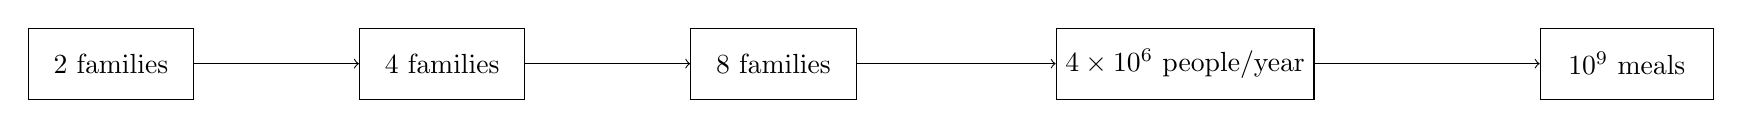
\begin{tikzpicture}[x=2.55cm,y=1.1cm]
\node[draw,rectangle,minimum width=2.1cm,minimum height=0.9cm] (a) at (0,0) {$2$ families};
\node[draw,rectangle,minimum width=2.1cm,minimum height=0.9cm] (b) at (1.65,0) {$4$ families};
\node[draw,rectangle,minimum width=2.1cm,minimum height=0.9cm] (c) at (3.3,0) {$8$ families};
\node[draw,rectangle,minimum width=2.5cm,minimum height=0.9cm] (d) at (5.35,0) {$4\times 10^6$ people/year};
\node[draw,rectangle,minimum width=2.2cm,minimum height=0.9cm] (e) at (7.55,0) {$10^9$ meals};
\draw[->] (a) -- (b);
\draw[->] (b) -- (c);
\draw[->] (c) -- (d);
\draw[->] (d) -- (e);
\end{tikzpicture}
\caption{A transcript-backed reconstruction of Robbins's giving ladder. The crucial point is not a single unit of measurement but the repeated enlargement of scale.}
\end{figure}

What gives this passage its force is the inversion Robbins insists on. The life grows not by beginning with ``how do I get more?'' but by beginning with ``how do I give more?'' The lecture does not claim that generosity mechanically produces billions. It claims something subtler and stronger: giving reorganizes meaning, and a changed meaning reorganizes action.

\section{Tony Robbins: equal souls, unequal markets}

The lecture now raises its clearest conceptual obstacle. The host frames it through networking, mentorship, and a common slogan: people say it is not what you know but who you know. Yet what if one has little credibility and little to offer? Robbins answers by going back to Jim Rohn, and that move tightens the question. Why were good men in his own family always broke, while other people made vast sums in the same world?

\subsection{Question \& Answer}

\paragraph{Question.} If people are equal in dignity, why are they so unequal in the marketplace?

\paragraph{Answer.} Robbins preserves Jim Rohn's distinction almost verbatim: we are equal as souls, but not equal in the marketplace. The market does not price inward dignity. It prices usefulness and scale of contribution. A schematic reconstruction is
\begin{equation}
Y_2 = kY_1,\qquad k\in\{2,10,50\},
\end{equation}
with the relevant interval of time held fixed. Jim Rohn's answer is then compressed by Robbins into one principle:
\begin{equation}
Y \propto V_{\text{market}}.
\end{equation}
This is not a theorem stated by the lecture as mathematics. It is a faithful note-writer reconstruction of the spoken rule: if one wishes to be paid more, one must become more valuable to other people.

That same rule explains access. There was no social-media shortcut in Robbins's early period. He went to work for people, even as a janitor, simply to be near them, and then increased his access by adding value first:
\begin{equation}
\text{access} \to \text{add value} \to \text{more access}.
\end{equation}
The lecture is careful on this point. One does not give whatever one feels like giving. One gives what the other person actually needs. That is the marketplace version of service.

\begin{figure}[h]
\centering
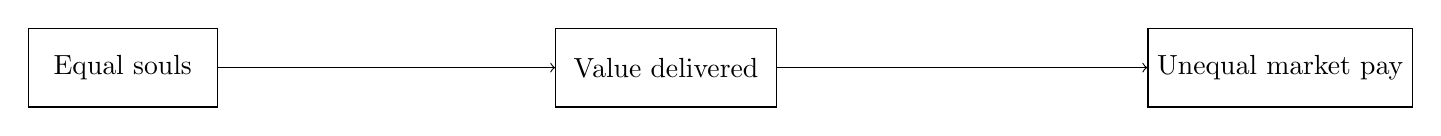
\begin{tikzpicture}[x=3.0cm,y=1.2cm]
\node[draw,rectangle,minimum width=2.4cm,minimum height=1.0cm] (a) at (0,0) {Equal souls};
\node[draw,rectangle,minimum width=2.8cm,minimum height=1.0cm] (b) at (2.3,0) {Value delivered};
\node[draw,rectangle,minimum width=2.9cm,minimum height=1.0cm] (c) at (4.9,0) {Unequal market pay};
\draw[->] (a) -- (b);
\draw[->] (b) -- (c);
\end{tikzpicture}
\caption{A transcript-backed reconstruction of the Jim Rohn distinction as Robbins retells it. Dignity is universal; market compensation is mediated by value delivered to others.}
\end{figure}

This is the section that prevents the chapter from turning into a mere collection of wealthy anecdotes. It gives a criterion. Once the lecture has posed the inequality problem, it refuses resentment as an explanation and replaces it with a harder and more operational question: what is being done for others, and at what scale?

\section{Fear, leverage, mission, and the Jake Paul coda}

From value the lecture moves to fear. Asked what he has learned about people, Robbins says that many prefer stories to confrontation. They tell themselves why their lives have not worked out rather than facing the fear that blocks movement. This produces one of the cleanest formal statements in the chapter:
\begin{equation}
\text{fearless} \neq \text{no fear}, \qquad
\text{courage} = \text{fear present} + \text{action anyway}.
\end{equation}
The wall that protects also imprisons. Thus the lecture's practical lesson is immediate: one does not wait for complete emotional cleanliness before acting.

The interview then returns to scale through Robbins's annual summit:
\begin{align}
N_{\text{summit}} &= 1.3\times 10^{6},\\
d &= 3,\\
h_{\text{day}} &\approx 2.5\ \text{hours},\\
N_{\text{LED}} &= 25,\\
H_{\text{ceiling}} &\approx 50\ \text{ft}.
\end{align}
These numbers prepare the next problem. How does one person travel, teach, maintain a family, and still sit inside 114 companies? Robbins's answer is that diversification comes late, not early. He admits he once wanted help with many opportunities too soon and was scolded by billionaire friends for trying to do twelve things before mastering one. The entrepreneur must not spread himself thin. First mastery, then leverage:
\begin{equation}
\text{operator} \to \text{owner} \to \text{leaders} \to \text{scale}.
\end{equation}
Hustle is useful at the beginning, but it is not the final architecture. The owner form requires strategic distance, strong leaders, and the ability to let other people carry real responsibility.

The last part of the Robbins interview adds the energy principle that holds the whole section together. One must become relentless, the creator of one's own life, and most of all the servant of something larger than oneself. If it is only about the self, the energy source is small. If it is about children, family, mission, or work that matters, the energy source becomes durable.

\subsection{Question \& Answer}

\paragraph{Question.} What does it mean to be fearless if fear never disappears?

\paragraph{Answer.} It means that fear is no longer the stopping condition. The lecture lowers the meaning of fearlessness and raises the meaning of action. One fears less, not zero. One acts anyway. Over repeated action the emotional range widens, and what had looked like a wall becomes only a threshold.

At this point the lecture deliberately repeats its opening rhythm. Dr.\ D reappears, Jake Paul access is again uncertain, credentials are again a problem, and the crew again hovers at the edge of being turned away. Only then does Jake Paul arrive. This recurrence matters. The chapter ends not by abandoning the field method, but by proving that the field method still governs the celebrity coda.

Jake Paul compresses several earlier doctrines into a newer idiom. He says the first million came at about age twenty and that investing began at eighteen. The early money came from YouTube views, brand deals, and merchandise; the later scale includes investing. Asked about a large year, he immediately insists that the number be counted net rather than gross:
\begin{equation}
Y_{\text{net}} < Y_{\text{gross}}.
\end{equation}
The inequality is obvious, but the discipline is not. The lecture wants us to hear the accounting sobriety in the statement ``always count the net.''

He then restates Robbins's fear doctrine almost point for point. Fear is present before the fight. Success lies outside the comfort zone. Negative thoughts are acknowledged like passing cars and then released. Vision matters. Fun matters because fun creates flow. Hatred from others is treated as projection from people living below the level of their own ambition. Finally, faith is named explicitly: God, prayer, and breathwork are not introduced as separate theology, but as supports for composure, courage, and persistence.

Thus the chapter closes as it began, with access, refusal, motion, and then an extracted rule. Jake Paul's last message is almost a compressed index of the whole lecture: find God, work hard, persevere, practice discipline, and do not organize your life around what others think.

\section{Summary}

This lecture is not mathematical in the blackboard sense, but it has a genuine mathematical spine. Palm Beach first teaches a method: approach, refusal, reset, renewed approach. The yacht owner supplies the first law: capital must move. The private-equity operator adds a sharper arithmetic: spending carries a replacement burden, saved capital is the entrance ticket to compounding, and follow-up preserves deals. Tony Robbins then supplies the larger frame: strangers can alter destiny, giving can scale, market compensation tracks value delivered rather than inward dignity, courage is action under fear, and real scale requires the movement from operator to owner. Jake Paul closes the loop by restating the same architecture in a younger register: net over gross, fear harnessed rather than denied, and discipline sustained by vision and faith.